% Options for packages loaded elsewhere
\PassOptionsToPackage{unicode}{hyperref}
\PassOptionsToPackage{hyphens}{url}
\PassOptionsToPackage{dvipsnames,svgnames,x11names}{xcolor}
%
\documentclass[
  letterpaper,
  DIV=11,
  numbers=noendperiod]{scrartcl}

\usepackage{amsmath,amssymb}
\usepackage{iftex}
\ifPDFTeX
  \usepackage[T1]{fontenc}
  \usepackage[utf8]{inputenc}
  \usepackage{textcomp} % provide euro and other symbols
\else % if luatex or xetex
  \usepackage{unicode-math}
  \defaultfontfeatures{Scale=MatchLowercase}
  \defaultfontfeatures[\rmfamily]{Ligatures=TeX,Scale=1}
\fi
\usepackage{lmodern}
\ifPDFTeX\else  
    % xetex/luatex font selection
\fi
% Use upquote if available, for straight quotes in verbatim environments
\IfFileExists{upquote.sty}{\usepackage{upquote}}{}
\IfFileExists{microtype.sty}{% use microtype if available
  \usepackage[]{microtype}
  \UseMicrotypeSet[protrusion]{basicmath} % disable protrusion for tt fonts
}{}
\makeatletter
\@ifundefined{KOMAClassName}{% if non-KOMA class
  \IfFileExists{parskip.sty}{%
    \usepackage{parskip}
  }{% else
    \setlength{\parindent}{0pt}
    \setlength{\parskip}{6pt plus 2pt minus 1pt}}
}{% if KOMA class
  \KOMAoptions{parskip=half}}
\makeatother
\usepackage{xcolor}
\setlength{\emergencystretch}{3em} % prevent overfull lines
\setcounter{secnumdepth}{-\maxdimen} % remove section numbering
% Make \paragraph and \subparagraph free-standing
\ifx\paragraph\undefined\else
  \let\oldparagraph\paragraph
  \renewcommand{\paragraph}[1]{\oldparagraph{#1}\mbox{}}
\fi
\ifx\subparagraph\undefined\else
  \let\oldsubparagraph\subparagraph
  \renewcommand{\subparagraph}[1]{\oldsubparagraph{#1}\mbox{}}
\fi

\usepackage{color}
\usepackage{fancyvrb}
\newcommand{\VerbBar}{|}
\newcommand{\VERB}{\Verb[commandchars=\\\{\}]}
\DefineVerbatimEnvironment{Highlighting}{Verbatim}{commandchars=\\\{\}}
% Add ',fontsize=\small' for more characters per line
\usepackage{framed}
\definecolor{shadecolor}{RGB}{241,243,245}
\newenvironment{Shaded}{\begin{snugshade}}{\end{snugshade}}
\newcommand{\AlertTok}[1]{\textcolor[rgb]{0.68,0.00,0.00}{#1}}
\newcommand{\AnnotationTok}[1]{\textcolor[rgb]{0.37,0.37,0.37}{#1}}
\newcommand{\AttributeTok}[1]{\textcolor[rgb]{0.40,0.45,0.13}{#1}}
\newcommand{\BaseNTok}[1]{\textcolor[rgb]{0.68,0.00,0.00}{#1}}
\newcommand{\BuiltInTok}[1]{\textcolor[rgb]{0.00,0.23,0.31}{#1}}
\newcommand{\CharTok}[1]{\textcolor[rgb]{0.13,0.47,0.30}{#1}}
\newcommand{\CommentTok}[1]{\textcolor[rgb]{0.37,0.37,0.37}{#1}}
\newcommand{\CommentVarTok}[1]{\textcolor[rgb]{0.37,0.37,0.37}{\textit{#1}}}
\newcommand{\ConstantTok}[1]{\textcolor[rgb]{0.56,0.35,0.01}{#1}}
\newcommand{\ControlFlowTok}[1]{\textcolor[rgb]{0.00,0.23,0.31}{#1}}
\newcommand{\DataTypeTok}[1]{\textcolor[rgb]{0.68,0.00,0.00}{#1}}
\newcommand{\DecValTok}[1]{\textcolor[rgb]{0.68,0.00,0.00}{#1}}
\newcommand{\DocumentationTok}[1]{\textcolor[rgb]{0.37,0.37,0.37}{\textit{#1}}}
\newcommand{\ErrorTok}[1]{\textcolor[rgb]{0.68,0.00,0.00}{#1}}
\newcommand{\ExtensionTok}[1]{\textcolor[rgb]{0.00,0.23,0.31}{#1}}
\newcommand{\FloatTok}[1]{\textcolor[rgb]{0.68,0.00,0.00}{#1}}
\newcommand{\FunctionTok}[1]{\textcolor[rgb]{0.28,0.35,0.67}{#1}}
\newcommand{\ImportTok}[1]{\textcolor[rgb]{0.00,0.46,0.62}{#1}}
\newcommand{\InformationTok}[1]{\textcolor[rgb]{0.37,0.37,0.37}{#1}}
\newcommand{\KeywordTok}[1]{\textcolor[rgb]{0.00,0.23,0.31}{#1}}
\newcommand{\NormalTok}[1]{\textcolor[rgb]{0.00,0.23,0.31}{#1}}
\newcommand{\OperatorTok}[1]{\textcolor[rgb]{0.37,0.37,0.37}{#1}}
\newcommand{\OtherTok}[1]{\textcolor[rgb]{0.00,0.23,0.31}{#1}}
\newcommand{\PreprocessorTok}[1]{\textcolor[rgb]{0.68,0.00,0.00}{#1}}
\newcommand{\RegionMarkerTok}[1]{\textcolor[rgb]{0.00,0.23,0.31}{#1}}
\newcommand{\SpecialCharTok}[1]{\textcolor[rgb]{0.37,0.37,0.37}{#1}}
\newcommand{\SpecialStringTok}[1]{\textcolor[rgb]{0.13,0.47,0.30}{#1}}
\newcommand{\StringTok}[1]{\textcolor[rgb]{0.13,0.47,0.30}{#1}}
\newcommand{\VariableTok}[1]{\textcolor[rgb]{0.07,0.07,0.07}{#1}}
\newcommand{\VerbatimStringTok}[1]{\textcolor[rgb]{0.13,0.47,0.30}{#1}}
\newcommand{\WarningTok}[1]{\textcolor[rgb]{0.37,0.37,0.37}{\textit{#1}}}

\providecommand{\tightlist}{%
  \setlength{\itemsep}{0pt}\setlength{\parskip}{0pt}}\usepackage{longtable,booktabs,array}
\usepackage{calc} % for calculating minipage widths
% Correct order of tables after \paragraph or \subparagraph
\usepackage{etoolbox}
\makeatletter
\patchcmd\longtable{\par}{\if@noskipsec\mbox{}\fi\par}{}{}
\makeatother
% Allow footnotes in longtable head/foot
\IfFileExists{footnotehyper.sty}{\usepackage{footnotehyper}}{\usepackage{footnote}}
\makesavenoteenv{longtable}
\usepackage{graphicx}
\makeatletter
\def\maxwidth{\ifdim\Gin@nat@width>\linewidth\linewidth\else\Gin@nat@width\fi}
\def\maxheight{\ifdim\Gin@nat@height>\textheight\textheight\else\Gin@nat@height\fi}
\makeatother
% Scale images if necessary, so that they will not overflow the page
% margins by default, and it is still possible to overwrite the defaults
% using explicit options in \includegraphics[width, height, ...]{}
\setkeys{Gin}{width=\maxwidth,height=\maxheight,keepaspectratio}
% Set default figure placement to htbp
\makeatletter
\def\fps@figure{htbp}
\makeatother

\usepackage{booktabs}
\usepackage{longtable}
\usepackage{array}
\usepackage{multirow}
\usepackage{wrapfig}
\usepackage{float}
\usepackage{colortbl}
\usepackage{pdflscape}
\usepackage{tabu}
\usepackage{threeparttable}
\usepackage{threeparttablex}
\usepackage[normalem]{ulem}
\usepackage{makecell}
\usepackage{xcolor}
\KOMAoption{captions}{tableheading}
\makeatletter
\makeatother
\makeatletter
\makeatother
\makeatletter
\@ifpackageloaded{caption}{}{\usepackage{caption}}
\AtBeginDocument{%
\ifdefined\contentsname
  \renewcommand*\contentsname{Table of contents}
\else
  \newcommand\contentsname{Table of contents}
\fi
\ifdefined\listfigurename
  \renewcommand*\listfigurename{List of Figures}
\else
  \newcommand\listfigurename{List of Figures}
\fi
\ifdefined\listtablename
  \renewcommand*\listtablename{List of Tables}
\else
  \newcommand\listtablename{List of Tables}
\fi
\ifdefined\figurename
  \renewcommand*\figurename{Figure}
\else
  \newcommand\figurename{Figure}
\fi
\ifdefined\tablename
  \renewcommand*\tablename{Table}
\else
  \newcommand\tablename{Table}
\fi
}
\@ifpackageloaded{float}{}{\usepackage{float}}
\floatstyle{ruled}
\@ifundefined{c@chapter}{\newfloat{codelisting}{h}{lop}}{\newfloat{codelisting}{h}{lop}[chapter]}
\floatname{codelisting}{Listing}
\newcommand*\listoflistings{\listof{codelisting}{List of Listings}}
\makeatother
\makeatletter
\@ifpackageloaded{caption}{}{\usepackage{caption}}
\@ifpackageloaded{subcaption}{}{\usepackage{subcaption}}
\makeatother
\makeatletter
\@ifpackageloaded{tcolorbox}{}{\usepackage[skins,breakable]{tcolorbox}}
\makeatother
\makeatletter
\@ifundefined{shadecolor}{\definecolor{shadecolor}{rgb}{.97, .97, .97}}
\makeatother
\makeatletter
\makeatother
\makeatletter
\makeatother
\ifLuaTeX
  \usepackage{selnolig}  % disable illegal ligatures
\fi
\IfFileExists{bookmark.sty}{\usepackage{bookmark}}{\usepackage{hyperref}}
\IfFileExists{xurl.sty}{\usepackage{xurl}}{} % add URL line breaks if available
\urlstyle{same} % disable monospaced font for URLs
\hypersetup{
  pdftitle={RNA-Seq Report},
  pdfauthor={Sameet Mehta},
  colorlinks=true,
  linkcolor={blue},
  filecolor={Maroon},
  citecolor={Blue},
  urlcolor={Blue},
  pdfcreator={LaTeX via pandoc}}

\title{RNA-Seq Report}
\author{Sameet Mehta}
\date{2023-09-27}

\begin{document}
\maketitle
\ifdefined\Shaded\renewenvironment{Shaded}{\begin{tcolorbox}[breakable, frame hidden, interior hidden, sharp corners, boxrule=0pt, enhanced, borderline west={3pt}{0pt}{shadecolor}]}{\end{tcolorbox}}\fi

\hypertarget{introduction}{%
\subsection{Introduction}\label{introduction}}

This is analysis report for differential gene expression analysis. The
data is described in the later sections. In this section we are setting
up the requirements for the analysis to happen correcty. We will import
packages and functions.

\begin{Shaded}
\begin{Highlighting}[]
\CommentTok{\# library(remotes)}
\CommentTok{\# remotes::install\_github("sameet/quartoReport")}

\FunctionTok{library}\NormalTok{(quartoReport)}
\CommentTok{\# use\_thresh \textless{}{-} 0.05 \# global threshold to use as alpha in the analysis}
\end{Highlighting}
\end{Shaded}

Please note that this package is currently under active development.
This status may change in the future. Currently this package is
\textbf{not} ready for production use. USE AT YOUR OWN RISK.

\hypertarget{qc-report}{%
\subsection{QC Report}\label{qc-report}}

We do not have a metrics file available so we will do not have a QC
section.

\hypertarget{analysis}{%
\subsection{Analysis}\label{analysis}}

The following sections detail how we ingest the data, prepare the data
and process the data for analysis.

\hypertarget{read-in-meta-data}{%
\subsubsection{Read in meta-data}\label{read-in-meta-data}}

Meta-data in this context the the description of the files. A method to
inform which samples bear which labels. Essentially it is a dicionary
that has a one -\textgreater{} many relation ship between conditions and
samples. But, it has one -\textgreater{} one relationshp between sample
and condition.

This step expects a tab-separated values file with 2 columns. We may
extend this to more conditions per sample in the future, but currently
we expect only 2 columns in this file. In the code we will rename these
columns to \texttt{sample}, and \texttt{condition}.

\begin{Shaded}
\begin{Highlighting}[]
\NormalTok{meta\_df }\OtherTok{\textless{}{-}} \FunctionTok{read\_meta\_data}\NormalTok{(params}\SpecialCharTok{$}\NormalTok{meta\_fn)}

\NormalTok{meta\_df }\SpecialCharTok{|\textgreater{}}
\NormalTok{  kableExtra}\SpecialCharTok{::}\FunctionTok{kbl}\NormalTok{(}\AttributeTok{booktabs =} \ConstantTok{TRUE}\NormalTok{) }\SpecialCharTok{|\textgreater{}}
\NormalTok{  kableExtra}\SpecialCharTok{::}\FunctionTok{kable\_styling}\NormalTok{(}\AttributeTok{bootstrap\_options =} \FunctionTok{c}\NormalTok{(}\StringTok{"condensed"}\NormalTok{, }\StringTok{"striped"}\NormalTok{),}
                \AttributeTok{latex\_options =} \FunctionTok{c}\NormalTok{(}\StringTok{"striped"}\NormalTok{))}
\end{Highlighting}
\end{Shaded}

\hypertarget{tbl-read_meta_data}{}
\begin{table}
\caption{\label{tbl-read_meta_data}The sample-sheet provided and being used in this analysis. }\tabularnewline

\centering
\begin{tabular}[t]{lll}
\toprule
  & sample & condition\\
\midrule
\cellcolor{gray!6}{12\_5-10\_FB} & \cellcolor{gray!6}{12\_5-10\_FB} & \cellcolor{gray!6}{WT\_FOREBRAIN}\\
12\_5-10\_SP & 12\_5-10\_SP & WT\_sub.pallum\\
\cellcolor{gray!6}{2\_5-8\_FB} & \cellcolor{gray!6}{2\_5-8\_FB} & \cellcolor{gray!6}{GSRW\_FOREBRAIN}\\
2\_5-8\_SP & 2\_5-8\_SP & GSRW\_sub.pallum\\
\cellcolor{gray!6}{3\_5-10\_FB} & \cellcolor{gray!6}{3\_5-10\_FB} & \cellcolor{gray!6}{GSRW\_FOREBRAIN}\\
\addlinespace
3\_5-10\_SP & 3\_5-10\_SP & GSRW\_sub.pallum\\
\cellcolor{gray!6}{3\_5-8\_SP} & \cellcolor{gray!6}{3\_5-8\_SP} & \cellcolor{gray!6}{GSRW\_sub.pallum}\\
5\_5-8\_FB & 5\_5-8\_FB & WT\_FOREBRAIN\\
\cellcolor{gray!6}{5\_5-8\_SP} & \cellcolor{gray!6}{5\_5-8\_SP} & \cellcolor{gray!6}{WT\_sub.pallum}\\
6\_5-8\_FB & 6\_5-8\_FB & WT\_FOREBRAIN\\
\addlinespace
\cellcolor{gray!6}{6\_5-8\_SP} & \cellcolor{gray!6}{6\_5-8\_SP} & \cellcolor{gray!6}{WT\_sub.pallum}\\
\bottomrule
\end{tabular}
\end{table}

\hypertarget{read-in-contrasts}{%
\subsubsection{Read in Contrasts}\label{read-in-contrasts}}

We will read in the contrasts here. These are the combinations that we
are going to use. If a \texttt{contrasts.txt} file is provided, we will
do calculations for only those comparisons. Otherwise, we will do all
pair-wise comparisons from the \texttt{condition} column in the
meta-data.

It is usually best practice to think through the analysis. It is
possible for a given analysis all conditions need to be compared against
each other. However, typically only a small sub-set of the comparisons
will be relevant. E.g. in a time series kind of experimental design the
goal is to study differences between two consecutive time points
serially. If there are many time points number of comparisons increase
exponentially.

Most experimental designs \textbf{do not have} hundreds of comparisons.

\begin{Shaded}
\begin{Highlighting}[]
\NormalTok{contrasts\_df }\OtherTok{\textless{}{-}} \FunctionTok{get\_contrasts}\NormalTok{(}\AttributeTok{fn =}\NormalTok{ params}\SpecialCharTok{$}\NormalTok{contrasts, }\AttributeTok{meta\_df =}\NormalTok{ meta\_df)}

\NormalTok{contrasts\_df }\SpecialCharTok{|\textgreater{}}
\NormalTok{  kableExtra}\SpecialCharTok{::}\FunctionTok{kbl}\NormalTok{(}\AttributeTok{booktabs =} \ConstantTok{TRUE}\NormalTok{) }\SpecialCharTok{|\textgreater{}}
\NormalTok{  kableExtra}\SpecialCharTok{::}\FunctionTok{kable\_styling}\NormalTok{(}\AttributeTok{bootstrap\_options =} \FunctionTok{c}\NormalTok{(}\StringTok{"condensed"}\NormalTok{, }\StringTok{"striped"}\NormalTok{),}
                \AttributeTok{latex\_options =} \FunctionTok{c}\NormalTok{(}\StringTok{"striped"}\NormalTok{))}
\end{Highlighting}
\end{Shaded}

\hypertarget{tbl-contrasts}{}
\begin{table}
\caption{\label{tbl-contrasts}The contrasts being used in this analysis. }\tabularnewline

\centering
\begin{tabular}[t]{ll}
\toprule
c1 & c2\\
\midrule
\cellcolor{gray!6}{WT\_FOREBRAIN} & \cellcolor{gray!6}{GSRW\_FOREBRAIN}\\
WT\_sub.pallum & GSRW\_sub.pallum\\
\bottomrule
\end{tabular}
\end{table}

\hypertarget{read-in-the-count-data}{%
\subsubsection{Read in the count data}\label{read-in-the-count-data}}

The RNA-Seq pipeline generates two count matrices, the transcript-level
count matrix, and gene-level count matrix. In this analysis we are going
to use the gene-level count matrix \emph{only}. Consequently, for the
smRNA-Seq analysis this will be either the ``mature'' smRNA counts, or
the ``hairpin'' smRNA counts.

By design the genes are listed according to their Ensembl gene IDs, or
other IDs. For most model organisms most of the genes have a real human
readable name, but for many non-standard model organisms not all genes
have a human readable name. We will be initially doing all the analysis
using Ensembl gene IDs, and then annotate only the significantly changed
genes for most common model organisms e.g.~human, mouse, rat, drosophila
etc.

\begin{Shaded}
\begin{Highlighting}[]
\NormalTok{count\_mat }\OtherTok{\textless{}{-}} \FunctionTok{read\_count\_mat}\NormalTok{(}\AttributeTok{fn =}\NormalTok{ params}\SpecialCharTok{$}\NormalTok{counts, meta\_df)}
\end{Highlighting}
\end{Shaded}

\hypertarget{gene-expression-analysis}{%
\subsection{Gene Expression Analysis}\label{gene-expression-analysis}}

With the \texttt{DESeq2} method it is easier to generate the analysis
for all possible combinations as defined by the \texttt{condition}
column of the \texttt{meta\_df}. We can then extract the results for the
comparions of interest rather easily.

\begin{Shaded}
\begin{Highlighting}[]
\NormalTok{dds }\OtherTok{\textless{}{-}} \FunctionTok{make\_deseq\_object}\NormalTok{(}\AttributeTok{count\_mat =}\NormalTok{ count\_mat, }\AttributeTok{meta\_df =}\NormalTok{ meta\_df)}
\NormalTok{vs\_data }\OtherTok{\textless{}{-}} \FunctionTok{stabilize\_count\_data}\NormalTok{(dds)}
\end{Highlighting}
\end{Shaded}

It is advised that you save the \texttt{dds} object and the
\texttt{vs\_data} object. There are relatively expensive objects and
require sizable computation to generate. We want to preserve them in
case of further downstream analysis.

\begin{Shaded}
\begin{Highlighting}[]
\FunctionTok{save\_objects}\NormalTok{(dds, }\AttributeTok{op\_dir =}\NormalTok{ params}\SpecialCharTok{$}\NormalTok{outputs)}
\FunctionTok{save\_objects}\NormalTok{(vs\_data, }\AttributeTok{op\_dir =}\NormalTok{ params}\SpecialCharTok{$}\NormalTok{outputs)}
\end{Highlighting}
\end{Shaded}

The DESeqDataSet-\ldots{} file represents the DESeq data-set that will
be used in this analysis. The DESEqTransform-\ldots{} file represents a
\texttt{vst}-transformed count data file. The files will be saved in
output directory defined in the \texttt{params} section of the
\texttt{YAML}.

\hypertarget{results-for-comparison-wt_forebraingsrw_forebrain}{%
\subsection{Results for comparison
WT\_FOREBRAIN--GSRW\_FOREBRAIN}\label{results-for-comparison-wt_forebraingsrw_forebrain}}

This comparison has a total of 398 s{[}1{]}
``qmd/sample\_report\_trial.qmd'' report we will show informatin about
top 30 genes.

\hypertarget{changed-genes-for-wt_forebraingsrw_forebrain}{%
\subsubsection{Changed genes for
WT\_FOREBRAIN--GSRW\_FOREBRAIN}\label{changed-genes-for-wt_forebraingsrw_forebrain}}

In Table~\ref{tbl-comparison_1} we see top genes changed between
WT\_FOREBRAIN--GSRW\_FOREBRAIN.

\begin{Shaded}
\begin{Highlighting}[]
\NormalTok{res\_df\_1 }\OtherTok{\textless{}{-}} \FunctionTok{get\_single\_result}\NormalTok{(dds, }\AttributeTok{comp\_df =}\NormalTok{ contrasts\_df[}\DecValTok{1}\NormalTok{, ])}
\NormalTok{res\_df\_1 }\SpecialCharTok{|\textgreater{}}
\NormalTok{  dplyr}\SpecialCharTok{::}\FunctionTok{filter}\NormalTok{(padj }\SpecialCharTok{\textless{}=} \FloatTok{0.05}\NormalTok{) }\SpecialCharTok{|\textgreater{}}
\NormalTok{  dplyr}\SpecialCharTok{::}\FunctionTok{arrange}\NormalTok{(}\FunctionTok{desc}\NormalTok{(}\FunctionTok{abs}\NormalTok{(log2FoldChange))) }\SpecialCharTok{|\textgreater{}}
\NormalTok{  dplyr}\SpecialCharTok{::}\FunctionTok{slice\_max}\NormalTok{(}\AttributeTok{order\_by =} \FunctionTok{abs}\NormalTok{(log2FoldChange), }\AttributeTok{n =} \DecValTok{30}\NormalTok{) }\SpecialCharTok{|\textgreater{}}
\NormalTok{  dplyr}\SpecialCharTok{::}\FunctionTok{arrange}\NormalTok{(}\FunctionTok{desc}\NormalTok{(log2FoldChange)) }\SpecialCharTok{|\textgreater{}}
\NormalTok{  dplyr}\SpecialCharTok{::}\FunctionTok{select}\NormalTok{(gene\_id, log2FoldChange, padj) }\OtherTok{{-}\textgreater{}}\NormalTok{ use\_sig\_df\_1}

\NormalTok{upreg\_rows }\OtherTok{\textless{}{-}} \FunctionTok{which}\NormalTok{(use\_sig\_df\_1}\SpecialCharTok{$}\NormalTok{log2FoldChange }\SpecialCharTok{\textgreater{}} \DecValTok{0}\NormalTok{)}
\NormalTok{downreg\_rows }\OtherTok{\textless{}{-}} \FunctionTok{which}\NormalTok{(use\_sig\_df\_1}\SpecialCharTok{$}\NormalTok{log2FoldChange }\SpecialCharTok{\textless{}} \DecValTok{0}\NormalTok{)}

\NormalTok{use\_sig\_df\_1 }\SpecialCharTok{|\textgreater{}}
\NormalTok{  kableExtra}\SpecialCharTok{::}\FunctionTok{kbl}\NormalTok{(}\AttributeTok{booktabs =} \ConstantTok{TRUE}\NormalTok{) }\SpecialCharTok{|\textgreater{}}
\NormalTok{  kableExtra}\SpecialCharTok{::}\FunctionTok{kable\_styling}\NormalTok{(}\AttributeTok{bootstrap\_options =} \FunctionTok{c}\NormalTok{(}\StringTok{"condensed"}\NormalTok{),}
                           \AttributeTok{latex\_options =} \FunctionTok{c}\NormalTok{(}\StringTok{"striped"}\NormalTok{),}
                           \AttributeTok{font\_size =} \DecValTok{8}
\NormalTok{                           ) }\SpecialCharTok{|\textgreater{}}
\NormalTok{  kableExtra}\SpecialCharTok{::}\FunctionTok{row\_spec}\NormalTok{(upreg\_rows, }\AttributeTok{color =} \StringTok{"red"}\NormalTok{) }\SpecialCharTok{|\textgreater{}}
\NormalTok{  kableExtra}\SpecialCharTok{::}\FunctionTok{row\_spec}\NormalTok{(downreg\_rows, }\AttributeTok{color =} \StringTok{"blue"}\NormalTok{)}
\end{Highlighting}
\end{Shaded}

\hypertarget{tbl-comparison_1}{}
\begin{table}
\caption{\label{tbl-comparison_1}Top changed differentially expressed genes in
WT\_FOREBRAIN--GSRW\_FOREBRAIN. }\tabularnewline

\centering\begingroup\fontsize{8}{10}\selectfont

\begin{tabular}[t]{lrr}
\toprule
gene\_id & log2FoldChange & padj\\
\midrule
\textcolor{red}{\cellcolor{gray!6}{mt-Ty}} & \textcolor{red}{\cellcolor{gray!6}{6.744684}} & \textcolor{red}{\cellcolor{gray!6}{0.0361441}}\\
\textcolor{red}{Tbx3os1} & \textcolor{red}{6.609995} & \textcolor{red}{0.0024765}\\
\textcolor{red}{\cellcolor{gray!6}{Gm3373}} & \textcolor{red}{\cellcolor{gray!6}{6.357571}} & \textcolor{red}{\cellcolor{gray!6}{0.0056723}}\\
\textcolor{red}{Syce1} & \textcolor{red}{6.330003} & \textcolor{red}{0.0084085}\\
\textcolor{red}{\cellcolor{gray!6}{Cfap221}} & \textcolor{red}{\cellcolor{gray!6}{6.173533}} & \textcolor{red}{\cellcolor{gray!6}{0.0116728}}\\
\addlinespace
\textcolor{red}{Lgals7} & \textcolor{red}{5.985162} & \textcolor{red}{0.0173271}\\
\textcolor{red}{\cellcolor{gray!6}{Krt19}} & \textcolor{red}{\cellcolor{gray!6}{5.799875}} & \textcolor{red}{\cellcolor{gray!6}{0.0261443}}\\
\textcolor{red}{Erich5} & \textcolor{red}{5.780783} & \textcolor{red}{0.0258869}\\
\textcolor{red}{\cellcolor{gray!6}{Trim10}} & \textcolor{red}{\cellcolor{gray!6}{5.744044}} & \textcolor{red}{\cellcolor{gray!6}{0.0295832}}\\
\textcolor{red}{Gm7901} & \textcolor{red}{5.569934} & \textcolor{red}{0.0000002}\\
\addlinespace
\textcolor{red}{\cellcolor{gray!6}{Ccdc178}} & \textcolor{red}{\cellcolor{gray!6}{5.448423}} & \textcolor{red}{\cellcolor{gray!6}{0.0343996}}\\
\textcolor{red}{AC135641.1} & \textcolor{red}{5.437715} & \textcolor{red}{0.0472750}\\
\textcolor{red}{\cellcolor{gray!6}{Tpm3-rs7}} & \textcolor{red}{\cellcolor{gray!6}{5.423427}} & \textcolor{red}{\cellcolor{gray!6}{0.0134045}}\\
\textcolor{blue}{B230323A14Rik} & \textcolor{blue}{-5.155336} & \textcolor{blue}{0.0085638}\\
\textcolor{blue}{\cellcolor{gray!6}{Gm28703}} & \textcolor{blue}{\cellcolor{gray!6}{-5.407426}} & \textcolor{blue}{\cellcolor{gray!6}{0.0295832}}\\
\addlinespace
\textcolor{blue}{Sall4} & \textcolor{blue}{-5.459355} & \textcolor{blue}{0.0277259}\\
\textcolor{blue}{\cellcolor{gray!6}{Tex38}} & \textcolor{blue}{\cellcolor{gray!6}{-5.520092}} & \textcolor{blue}{\cellcolor{gray!6}{0.0277259}}\\
\textcolor{blue}{Slc25a21} & \textcolor{blue}{-5.525488} & \textcolor{blue}{0.0237072}\\
\textcolor{blue}{\cellcolor{gray!6}{Mobp}} & \textcolor{blue}{\cellcolor{gray!6}{-5.739904}} & \textcolor{blue}{\cellcolor{gray!6}{0.0195807}}\\
\textcolor{blue}{Gm26812} & \textcolor{blue}{-5.780755} & \textcolor{blue}{0.0028014}\\
\addlinespace
\textcolor{blue}{\cellcolor{gray!6}{Cyb5r2}} & \textcolor{blue}{\cellcolor{gray!6}{-5.964004}} & \textcolor{blue}{\cellcolor{gray!6}{0.0149785}}\\
\textcolor{blue}{Ppp1r1c} & \textcolor{blue}{-6.051918} & \textcolor{blue}{0.0004003}\\
\textcolor{blue}{\cellcolor{gray!6}{Lrrc39}} & \textcolor{blue}{\cellcolor{gray!6}{-6.057120}} & \textcolor{blue}{\cellcolor{gray!6}{0.0496973}}\\
\textcolor{blue}{Slfn4} & \textcolor{blue}{-6.110792} & \textcolor{blue}{0.0357404}\\
\textcolor{blue}{\cellcolor{gray!6}{Adgb}} & \textcolor{blue}{\cellcolor{gray!6}{-6.342525}} & \textcolor{blue}{\cellcolor{gray!6}{0.0100377}}\\
\addlinespace
\textcolor{blue}{Slc6a5} & \textcolor{blue}{-6.521675} & \textcolor{blue}{0.0128507}\\
\textcolor{blue}{\cellcolor{gray!6}{2610028E06Rik}} & \textcolor{blue}{\cellcolor{gray!6}{-6.722017}} & \textcolor{blue}{\cellcolor{gray!6}{0.0006642}}\\
\textcolor{blue}{Eci3} & \textcolor{blue}{-7.603867} & \textcolor{blue}{0.0000915}\\
\textcolor{blue}{\cellcolor{gray!6}{Xist}} & \textcolor{blue}{\cellcolor{gray!6}{-11.984433}} & \textcolor{blue}{\cellcolor{gray!6}{0.0000468}}\\
\textcolor{blue}{Gm42047} & \textcolor{blue}{-13.319121} & \textcolor{blue}{0.0000000}\\
\bottomrule
\end{tabular}
\endgroup{}
\end{table}

\hypertarget{data-visualization-for-wt_forebraingsrw_forebrain}{%
\subsubsection{Data Visualization for
WT\_FOREBRAIN--GSRW\_FOREBRAIN}\label{data-visualization-for-wt_forebraingsrw_forebrain}}

\begin{Shaded}
\begin{Highlighting}[]
\NormalTok{all\_plot\_1}\SpecialCharTok{$}\NormalTok{volcano}
\end{Highlighting}
\end{Shaded}

\begin{figure}[H]

{\centering 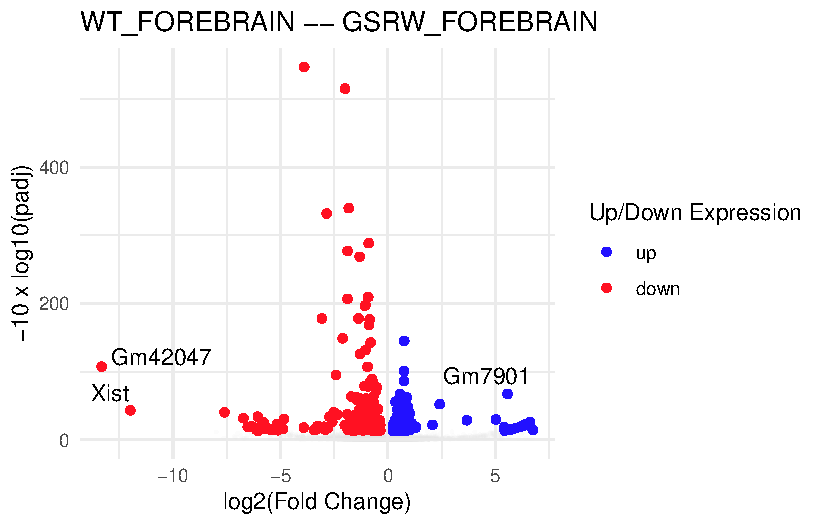
\includegraphics{sample_report_trial_files/figure-pdf/fig-volcano_1-1.pdf}

}

\caption{\label{fig-volcano_1}Volcano Plot for
WT\_FOREBRAIN--GSRW\_FOREBRAIN. Genes in blue are down-regulated, and
genes in red are up-regulated.}

\end{figure}

\begin{Shaded}
\begin{Highlighting}[]
\NormalTok{all\_plot\_1}\SpecialCharTok{$}\NormalTok{bp\_s}
\end{Highlighting}
\end{Shaded}

\begin{figure}[H]

{\centering 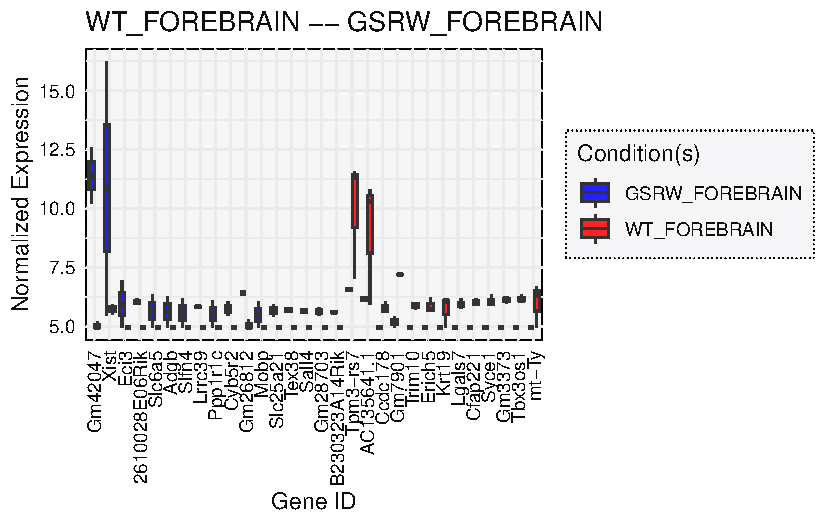
\includegraphics{sample_report_trial_files/figure-pdf/fig-boxplot_single_1-1.pdf}

}

\caption{\label{fig-boxplot_single_1}Boxplot for
WT\_FOREBRAIN--GSRW\_FOREBRAIN.}

\end{figure}

\begin{Shaded}
\begin{Highlighting}[]
\NormalTok{ggplotify}\SpecialCharTok{::}\FunctionTok{as.ggplot}\NormalTok{(all\_plot\_1}\SpecialCharTok{$}\NormalTok{hm)}
\end{Highlighting}
\end{Shaded}

\begin{figure}[H]

{\centering 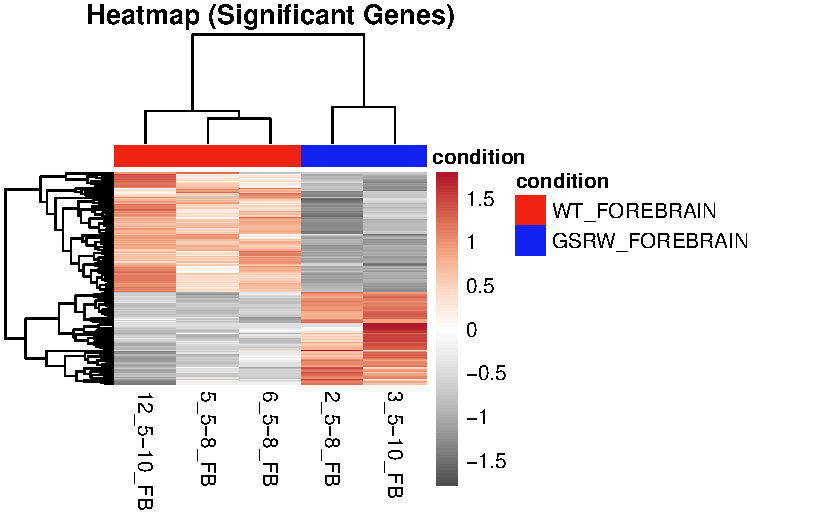
\includegraphics{sample_report_trial_files/figure-pdf/fig-hm_1-1.pdf}

}

\caption{\label{fig-hm_1}Heatmp for all significant genes for
WT\_FOREBRAIN--GSRW\_FOREBRAIN. There are total
\texttt{r\ nrow(sig\_df)} significant genes.}

\end{figure}

\hypertarget{results-for-comparison-wt_sub.pallumgsrw_sub.pallum}{%
\subsection{Results for comparison
WT\_sub.pallum--GSRW\_sub.pallum}\label{results-for-comparison-wt_sub.pallumgsrw_sub.pallum}}

This comparison has a total of 51 significant genes. Of those in this
report we will show informatin about top 30 genes.

\hypertarget{changed-genes-for-wt_sub.pallumgsrw_sub.pallum}{%
\subsubsection{Changed genes for
WT\_sub.pallum--GSRW\_sub.pallum}\label{changed-genes-for-wt_sub.pallumgsrw_sub.pallum}}

In Table~\ref{tbl-comparison_2} we see top genes changed between
WT\_sub.pallum--GSRW\_sub.pallum.

\begin{Shaded}
\begin{Highlighting}[]
\NormalTok{res\_df\_2 }\OtherTok{\textless{}{-}} \FunctionTok{get\_single\_result}\NormalTok{(dds, }\AttributeTok{comp\_df =}\NormalTok{ contrasts\_df[}\DecValTok{2}\NormalTok{, ])}
\NormalTok{res\_df\_2 }\SpecialCharTok{|\textgreater{}}
\NormalTok{  dplyr}\SpecialCharTok{::}\FunctionTok{filter}\NormalTok{(padj }\SpecialCharTok{\textless{}=} \FloatTok{0.05}\NormalTok{) }\SpecialCharTok{|\textgreater{}}
\NormalTok{  dplyr}\SpecialCharTok{::}\FunctionTok{arrange}\NormalTok{(}\FunctionTok{desc}\NormalTok{(}\FunctionTok{abs}\NormalTok{(log2FoldChange))) }\SpecialCharTok{|\textgreater{}}
\NormalTok{  dplyr}\SpecialCharTok{::}\FunctionTok{slice\_max}\NormalTok{(}\AttributeTok{order\_by =} \FunctionTok{abs}\NormalTok{(log2FoldChange), }\AttributeTok{n =} \DecValTok{30}\NormalTok{) }\SpecialCharTok{|\textgreater{}}
\NormalTok{  dplyr}\SpecialCharTok{::}\FunctionTok{arrange}\NormalTok{(}\FunctionTok{desc}\NormalTok{(log2FoldChange)) }\SpecialCharTok{|\textgreater{}}
\NormalTok{  dplyr}\SpecialCharTok{::}\FunctionTok{select}\NormalTok{(gene\_id, log2FoldChange, padj) }\OtherTok{{-}\textgreater{}}\NormalTok{ use\_sig\_df\_2}

\NormalTok{upreg\_rows }\OtherTok{\textless{}{-}} \FunctionTok{which}\NormalTok{(use\_sig\_df\_2}\SpecialCharTok{$}\NormalTok{log2FoldChange }\SpecialCharTok{\textgreater{}} \DecValTok{0}\NormalTok{)}
\NormalTok{downreg\_rows }\OtherTok{\textless{}{-}} \FunctionTok{which}\NormalTok{(use\_sig\_df\_2}\SpecialCharTok{$}\NormalTok{log2FoldChange }\SpecialCharTok{\textless{}} \DecValTok{0}\NormalTok{)}

\NormalTok{use\_sig\_df\_2 }\SpecialCharTok{|\textgreater{}}
\NormalTok{  kableExtra}\SpecialCharTok{::}\FunctionTok{kbl}\NormalTok{(}\AttributeTok{booktabs =} \ConstantTok{TRUE}\NormalTok{) }\SpecialCharTok{|\textgreater{}}
\NormalTok{  kableExtra}\SpecialCharTok{::}\FunctionTok{kable\_styling}\NormalTok{(}\AttributeTok{bootstrap\_options =} \FunctionTok{c}\NormalTok{(}\StringTok{"condensed"}\NormalTok{),}
                           \AttributeTok{latex\_options =} \FunctionTok{c}\NormalTok{(}\StringTok{"striped"}\NormalTok{),}
                           \AttributeTok{font\_size =} \DecValTok{8}
\NormalTok{                           ) }\SpecialCharTok{|\textgreater{}}
\NormalTok{  kableExtra}\SpecialCharTok{::}\FunctionTok{row\_spec}\NormalTok{(upreg\_rows, }\AttributeTok{color =} \StringTok{"red"}\NormalTok{) }\SpecialCharTok{|\textgreater{}}
\NormalTok{  kableExtra}\SpecialCharTok{::}\FunctionTok{row\_spec}\NormalTok{(downreg\_rows, }\AttributeTok{color =} \StringTok{"blue"}\NormalTok{)}
\end{Highlighting}
\end{Shaded}

\hypertarget{tbl-comparison_2}{}
\begin{table}
\caption{\label{tbl-comparison_2}Top changed differentially expressed genes in
WT\_sub.pallum--GSRW\_sub.pallum. }\tabularnewline

\centering\begingroup\fontsize{8}{10}\selectfont

\begin{tabular}[t]{lrr}
\toprule
gene\_id & log2FoldChange & padj\\
\midrule
\textcolor{red}{\cellcolor{gray!6}{AC135641.1}} & \textcolor{red}{\cellcolor{gray!6}{5.9024901}} & \textcolor{red}{\cellcolor{gray!6}{0.0300606}}\\
\textcolor{red}{Gm7901} & \textcolor{red}{5.4869687} & \textcolor{red}{0.0000000}\\
\textcolor{red}{\cellcolor{gray!6}{C030018K13Rik}} & \textcolor{red}{\cellcolor{gray!6}{5.1745342}} & \textcolor{red}{\cellcolor{gray!6}{0.0371569}}\\
\textcolor{red}{Gm9347} & \textcolor{red}{4.2974447} & \textcolor{red}{0.0000000}\\
\textcolor{red}{\cellcolor{gray!6}{Cxcl14}} & \textcolor{red}{\cellcolor{gray!6}{0.7804630}} & \textcolor{red}{\cellcolor{gray!6}{0.0352495}}\\
\addlinespace
\textcolor{blue}{Yars} & \textcolor{blue}{-0.6502437} & \textcolor{blue}{0.0000000}\\
\textcolor{blue}{\cellcolor{gray!6}{Mars}} & \textcolor{blue}{\cellcolor{gray!6}{-0.6584464}} & \textcolor{blue}{\cellcolor{gray!6}{0.0000000}}\\
\textcolor{blue}{Aldh18a1} & \textcolor{blue}{-0.6793612} & \textcolor{blue}{0.0000000}\\
\textcolor{blue}{\cellcolor{gray!6}{Phgdh}} & \textcolor{blue}{\cellcolor{gray!6}{-0.6999350}} & \textcolor{blue}{\cellcolor{gray!6}{0.0000001}}\\
\textcolor{blue}{Psat1} & \textcolor{blue}{-0.7274429} & \textcolor{blue}{0.0000001}\\
\addlinespace
\textcolor{blue}{\cellcolor{gray!6}{Gmnc}} & \textcolor{blue}{\cellcolor{gray!6}{-0.7695529}} & \textcolor{blue}{\cellcolor{gray!6}{0.0208708}}\\
\textcolor{blue}{Psph} & \textcolor{blue}{-0.7802286} & \textcolor{blue}{0.0000293}\\
\textcolor{blue}{\cellcolor{gray!6}{Ddit3}} & \textcolor{blue}{\cellcolor{gray!6}{-0.7898461}} & \textcolor{blue}{\cellcolor{gray!6}{0.0000182}}\\
\textcolor{blue}{1700048O20Rik} & \textcolor{blue}{-0.8447872} & \textcolor{blue}{0.0012956}\\
\textcolor{blue}{\cellcolor{gray!6}{Trim66}} & \textcolor{blue}{\cellcolor{gray!6}{-0.9176471}} & \textcolor{blue}{\cellcolor{gray!6}{0.0005239}}\\
\addlinespace
\textcolor{blue}{Aldh1l2} & \textcolor{blue}{-0.9588941} & \textcolor{blue}{0.0000000}\\
\textcolor{blue}{\cellcolor{gray!6}{Stc2}} & \textcolor{blue}{\cellcolor{gray!6}{-0.9630760}} & \textcolor{blue}{\cellcolor{gray!6}{0.0000001}}\\
\textcolor{blue}{Sesn2} & \textcolor{blue}{-0.9955183} & \textcolor{blue}{0.0009149}\\
\textcolor{blue}{\cellcolor{gray!6}{Atf4}} & \textcolor{blue}{\cellcolor{gray!6}{-1.0043621}} & \textcolor{blue}{\cellcolor{gray!6}{0.0000000}}\\
\textcolor{blue}{Asns} & \textcolor{blue}{-1.0432825} & \textcolor{blue}{0.0000000}\\
\addlinespace
\textcolor{blue}{\cellcolor{gray!6}{Cars}} & \textcolor{blue}{\cellcolor{gray!6}{-1.0682913}} & \textcolor{blue}{\cellcolor{gray!6}{0.0000000}}\\
\textcolor{blue}{Serpinf1} & \textcolor{blue}{-1.1245828} & \textcolor{blue}{0.0008941}\\
\textcolor{blue}{\cellcolor{gray!6}{Mthfd2}} & \textcolor{blue}{\cellcolor{gray!6}{-1.3152156}} & \textcolor{blue}{\cellcolor{gray!6}{0.0000000}}\\
\textcolor{blue}{P2rx3} & \textcolor{blue}{-1.4286902} & \textcolor{blue}{0.0046721}\\
\textcolor{blue}{\cellcolor{gray!6}{Atf5}} & \textcolor{blue}{\cellcolor{gray!6}{-1.5260532}} & \textcolor{blue}{\cellcolor{gray!6}{0.0000000}}\\
\addlinespace
\textcolor{blue}{Chac1} & \textcolor{blue}{-1.5841872} & \textcolor{blue}{0.0000088}\\
\textcolor{blue}{\cellcolor{gray!6}{Eif4ebp1}} & \textcolor{blue}{\cellcolor{gray!6}{-1.7103201}} & \textcolor{blue}{\cellcolor{gray!6}{0.0000182}}\\
\textcolor{blue}{Slc7a3} & \textcolor{blue}{-2.3024280} & \textcolor{blue}{0.0000000}\\
\textcolor{blue}{\cellcolor{gray!6}{Xist}} & \textcolor{blue}{\cellcolor{gray!6}{-11.8212319}} & \textcolor{blue}{\cellcolor{gray!6}{0.0000088}}\\
\textcolor{blue}{Gm42047} & \textcolor{blue}{-13.1200451} & \textcolor{blue}{0.0000000}\\
\bottomrule
\end{tabular}
\endgroup{}
\end{table}

\hypertarget{data-visualization-for-wt_sub.pallumgsrw_sub.pallum}{%
\subsubsection{Data Visualization for
WT\_sub.pallum--GSRW\_sub.pallum}\label{data-visualization-for-wt_sub.pallumgsrw_sub.pallum}}

\begin{Shaded}
\begin{Highlighting}[]
\NormalTok{all\_plot\_2}\SpecialCharTok{$}\NormalTok{volcano}
\end{Highlighting}
\end{Shaded}

\begin{figure}[H]

{\centering 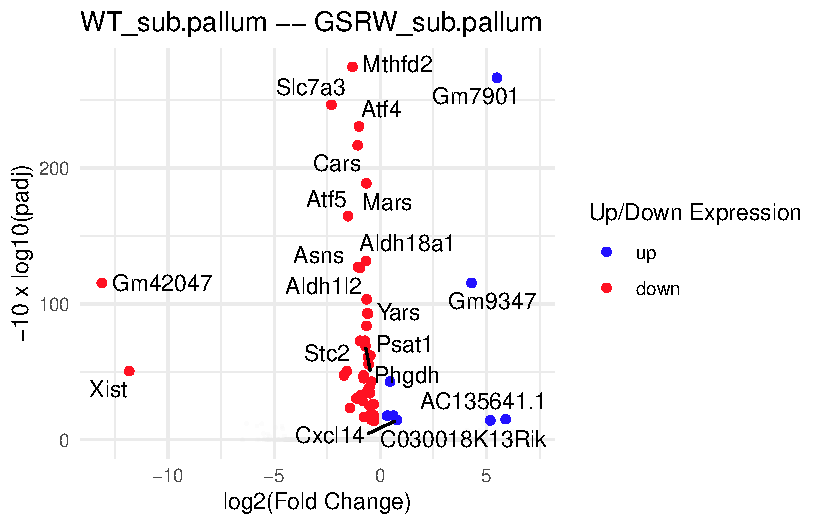
\includegraphics{sample_report_trial_files/figure-pdf/fig-volcano_2-1.pdf}

}

\caption{\label{fig-volcano_2}Volcano Plot for
WT\_sub.pallum--GSRW\_sub.pallum. Genes in blue are down-regulated, and
genes in red are up-regulated.}

\end{figure}

\begin{Shaded}
\begin{Highlighting}[]
\NormalTok{all\_plot\_2}\SpecialCharTok{$}\NormalTok{bp\_s}
\end{Highlighting}
\end{Shaded}

\begin{figure}[H]

{\centering 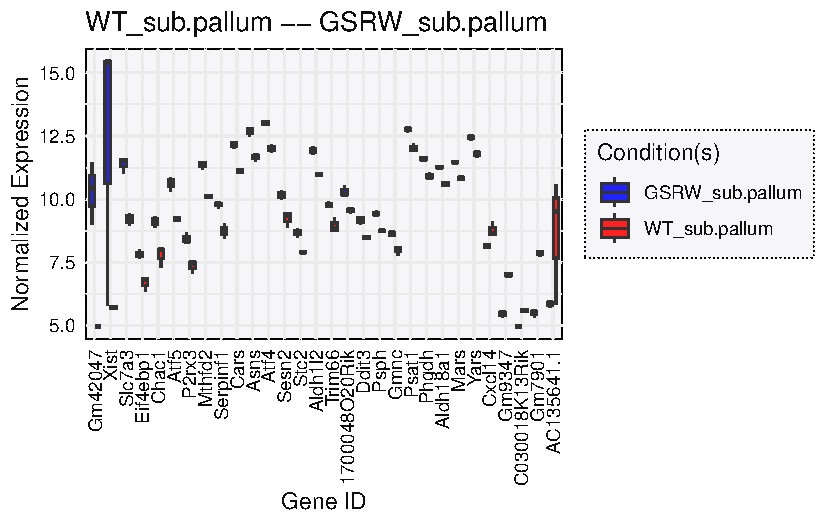
\includegraphics{sample_report_trial_files/figure-pdf/fig-boxplot_single_2-1.pdf}

}

\caption{\label{fig-boxplot_single_2}Boxplot for
WT\_sub.pallum--GSRW\_sub.pallum.}

\end{figure}

\begin{Shaded}
\begin{Highlighting}[]
\NormalTok{ggplotify}\SpecialCharTok{::}\FunctionTok{as.ggplot}\NormalTok{(all\_plot\_2}\SpecialCharTok{$}\NormalTok{hm)}
\end{Highlighting}
\end{Shaded}

\begin{figure}[H]

{\centering 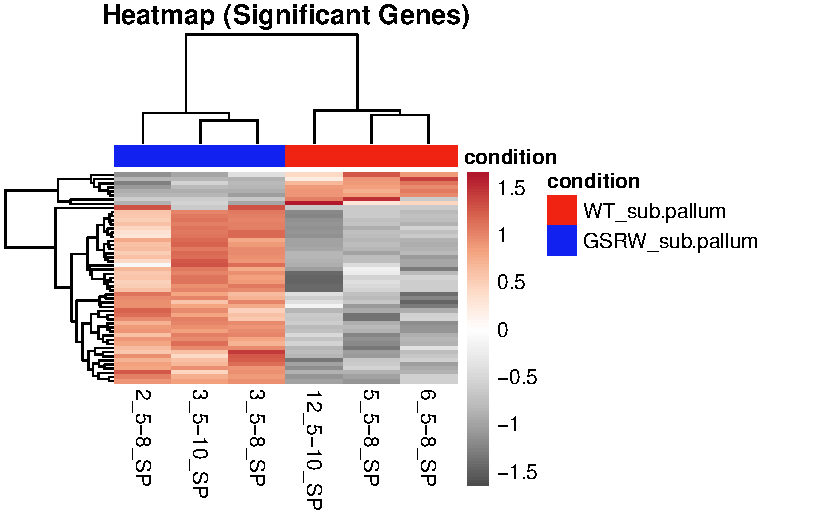
\includegraphics{sample_report_trial_files/figure-pdf/fig-hm_2-1.pdf}

}

\caption{\label{fig-hm_2}Heatmp for all significant genes for
WT\_sub.pallum--GSRW\_sub.pallum. There are total
\texttt{r\ nrow(sig\_df)} significant genes.}

\end{figure}



\end{document}
